\documentclass[14pt]{beamer}

\mode<presentation>{ \usetheme{Madrid}

% To remove the navigation symbols from the bottom of all slides uncomment next line
\setbeamertemplate{navigation symbols}{}
\date{}
\title{}
\author{}

%to get rid of footer entirely uncomment next line
\setbeamertemplate{footline}{}
}

\usepackage{geometry}
\usepackage{multirow}
\usepackage{adjustbox}
\usepackage{multicol}
\setlength{\columnsep}{0.1cm}

\usepackage{tikz}
\usetikzlibrary{shapes, backgrounds}

\usepackage{bbding}
\usepackage{rotating}
\usepackage{xcolor}

%\usepackage{tkz-berge} %cool grid
\usepackage{pgfplots} %pics

\usepackage{graphicx} % Allows including images
\usepackage{
	booktabs
} % Allows the use of \toprule, \midrule and \bottomrule in tables
\usepackage{mathtools}

\newcommand{\R}{\mathbb{R}}
\newcommand{\Z}{\mathbb{Z}}
\newcommand{\N}{\mathbb{N}}
\newcommand{\e}{\varepsilon}

\newcommand{\p}{% \pause
}

% simple environrment for enumerate, easier to read
\setbeamertemplate{enumerate items}[default]

%%%%%%%%%%%%%%%%%%%%%%

% to use colours easily
\definecolor{verde}{rgb}{0, .8, 0}
\definecolor{rosa}{rgb}{1, 0, 1}
\definecolor{naranja}{rgb}{1, .5, 0.1}
\newcommand{\azul}[1]{{\color{blue} #1}}
\newcommand{\rojo}[1]{{\color{red} #1}}
\newcommand{\verde}[1]{{\color{verde} #1}}
\newcommand{\rosa}[1]{{\color{rosa} #1}}
\newcommand{\naranja}[1]{{\color{naranja} #1}}
\newcommand{\violeta}[1]{{\color{violet} #1}}

% box in red and blue in math and outside of math
\newcommand{\cajar}[1]{\boxed{\mbox{\rojo{ #1}}}}
\newcommand{\majar}[1]{\boxed{\rojo{ #1}}}
\newcommand{\cajab}[1]{\boxed{\mbox{\azul{ #1}}}}
\newcommand{\majab}[1]{\boxed{\azul{ #1}}}

\newcommand{\setsize}[1]{\fontsize{#1}{#1}\selectfont} %allows you to change the font size. The default size of this document is 14. To change the font size of the whole slide, place this at the beginning of the slide. To change the size of only a portion of the text to size 12, you can do the following { \setsize{12} Your text. }.

\setbeamerfont{frametitle}{size=\fontsize{15}{15}\selectfont}
\setbeamerfont{block title}{size=\fontsize{14}{14}\selectfont}

\newcommand{\smallerfont}{\setsize{13}} %place this at the beginning of a slide to set the font size of the entire slide to 13.

%===========================

% Preamble just for this file

%===========================

\newcommand{\arcsec}{\operatorname{arcsec}}

%===================================================
\begin{document}
	%===================================================

	%----------------------------------------------------------------------------------------

	%	Related rates problems

	%----------------------------------------------------------------------------------------

	%-----------------------------

	%QUESTION_INFO: {"unit":6,"question":0,"title":"Lake ripple","images":[]}
	\begin{frame}[t]
		\frametitle{Lake ripple}

		We drop a pebble into a lake. It produces a circular ripple. When the radius
		is $2$ meters and is increasing at a rate of $10cm/s$, at what rate is the area
		increasing?
	\end{frame}
	%-----------------------------

	%QUESTION_INFO: {"unit":6,"question":1,"title":"Sliding ladder","images":[]}
	\begin{frame}[t]
		\frametitle{Sliding ladder}

		A ten-meter long ladder is leaning against a vertical wall and sliding. The top
		end of the ladder is 8 meters high and sliding down at a rate of 1 meter per
		second. At which rate is the bottom end sliding?
	\end{frame}
	%-----------------------------

	%QUESTION_INFO: {"unit":6,"question":2,"title":"Math party","images":[]}
	\begin{frame}[t]
		\frametitle{Math party}

		The MAT137 TAs wanted to rent a disco ball for their upcoming party. However,
		since they are poor, they could only afford a flashlight. At the party, one TA
		is designated the ``human disco ball''. The TA stands in the center of the
		room pointing the flashlight horizontally and spins at 3 revolutions per
		second. (Yes, they are that fast. Ask your TA to demonstratel if you don't
		believe me!) The room is square with side length 8 meters. At which speed is
		the light from the flashlight moving across the wall when it is 3 meters away
		from a corner?
	\end{frame}
	%-----------------------------

	%QUESTION_INFO: {"unit":6,"question":3,"title":"Sleepy ants","images":[]}
	\begin{frame}[t]
		\frametitle{Sleepy ants}

		Two ants are taking a nap. The first one is resting at the tip of the minute
		hand of a cuckoo clock, which is 25 cm long. The second one is resting at the
		tip of the hour hand, which is half the length. At what rate is the distance
		between the two ants changing at 3:30?
	\end{frame}
	%-----------------------------

	%QUESTION_INFO: {"unit":6,"question":4,"title":"The kite","images":[]}
	\begin{frame}[t]
		\frametitle{The kite}

		Mary Poppins is flying a kite. The kite is 21 meters above the ground and it
		is being blown horizontally by the wind at 2 m/s. Mary's hands are 1 meter
		above the ground. Right now 30 meters of string are out. At what rate is the
		string being released from Mary's hands?
	\end{frame}
	%-----------------------------

	%QUESTION_INFO: {"unit":6,"question":5,"title":"Coffee","images":[]}
	\begin{frame}[t]
		\frametitle{Coffee}

		A coffee filter is shaped like an inverted cone. It has a radius at the top of
		$4cm$ and it is $6cm$ in height. Coffee flows out of at the bottom at a rate
		of $2cm^{3}/s$. If the filter begins completely filled, how fast is the
		coffee level decreasing after 30 seconds?
	\end{frame}
	%-----------------------------

	%----------------------------------------------------------------------------------------

	%	Applied optimization problems

	%----------------------------------------------------------------------------------------

	%-----------------------------

	%QUESTION_INFO: {"unit":6,"question":6,"title":"The classic farmer problem","images":[]}
	\begin{frame}[t]
		\frametitle{The classic farmer problem}

		A farmer has $300m$ of fencing and wants to fence off a rectangular field
		and add an extra fence that divides the rectangular area in two equal parts
		down the middle. What is the largest area that the field can have?
	\end{frame}

	%-----------------------------

	%QUESTION_INFO: {"unit":6,"question":7,"title":"Distance","images":[]}
	\begin{frame}[t]
		\frametitle{Distance}

		Find the point on the parabola $y^{2}=2x$ that is closest to the point
		$(1,4)$.
	\end{frame}
	%-----------------------------

	%QUESTION_INFO: {"unit":6,"question":8,"title":"A matter of perspective","images":[]}
	\begin{frame}[t]
		\frametitle{A matter of perspective}

		A painting in an art gallery has height $h$ and is hung so that its lower
		edge is a distance $a$ above your eye. How far from the wall should you stand
		to get the best view?
	\end{frame}
	%-----------------------------

	%QUESTION_INFO: {"unit":6,"question":9,"title":"Airplane","images":[]}
	\begin{frame}[t]
		\frametitle{Airplane}

		The cost of fuel per hour for a certain airplane is proportional to the
		square of its speed and is \$1200 per hour for a speed of 600$km/h$. After every
		5,000 hours flown, the aircraft must undergo an \$8 million dollar safety inspection.
		What speed should the airplane fly at in order to achieve the lowest cost
		per kilometre?
	\end{frame}
	%-----------------------------

	%QUESTION_INFO: {"unit":6,"question":10,"title":"Fire","images":[]}
	\begin{frame}[t]
		\frametitle{Fire}

		You hear a scream. You turn around and you see Alfonso is on fire. Literally!
		Luckily, you are next to a straight river. Alfonso is 10 meters away from the
		river and you are 5 meters away from the point $P$ on the river closest to Alfonso.
		You are carrying an empty bucket. You can run twice as fast with an empty bucket
		as you can run with a full bucket. How far from the point P should you fill
		your bucket in order to get to Alfonso with a bucket full of water as fast
		as possible?

		% Warning!  This problem is a trap.  If you model it carelessly, it has  a critical point but it is outside the domain.
	\end{frame}
	%-----------------------------

	%QUESTION_INFO: {"unit":6,"question":11,"title":"Dominion","images":[]}
	\begin{frame}[t]
		\frametitle{Dominion}

		Dominion is a board game where, among other things, players buy cards worth
		victory points. The player with the most victory points wins.

		It is your last turn and you can only buy ``duchies'' and ``dukes''. A duchy
		is worth 3 victory points. A duke is worth as many victory points as duchies
		you have. Each duchy costs 3 coins, and each duke costs 3 coins. You have
		not bough any duke or duchy yet.

		If you have $N$ coins, how many dukes and how many duchies should you buy?
	\end{frame}
	%-----------------------------

	%----------------------------------------------------------------------------------------

	%	Indeterminate forms and L'H^{o}pital's Rule

	%----------------------------------------------------------------------------------------

	%-----------------------------

	%QUESTION_INFO: {"unit":6,"question":12,"title":"Limits from graphs","images":["G15.pdf","G14.pdf"]}
	\begin{frame}[t]
		\frametitle{Limits from graphs}

		Compute:

		\begin{multicols}{2}
			\begin{enumerate}
				\item $\displaystyle \lim_{x\to 0 }\frac{H(x)}{H(2+3x) - 1}$

				\item $\displaystyle \lim_{x \to 2}\frac{F^{-1}(x)}{x-2}$
			\end{enumerate}
		\end{multicols}

		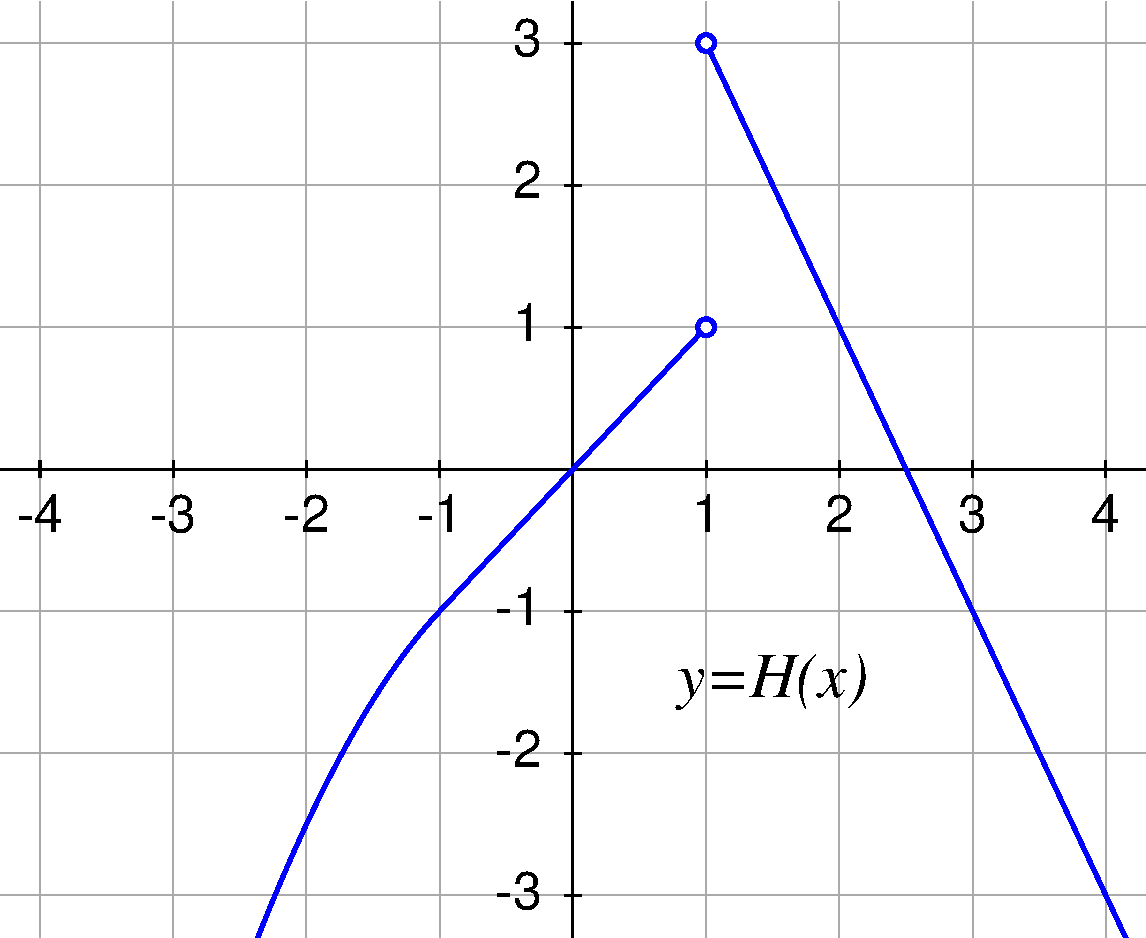
\includegraphics[scale=.29]{G14}
		\hfill
		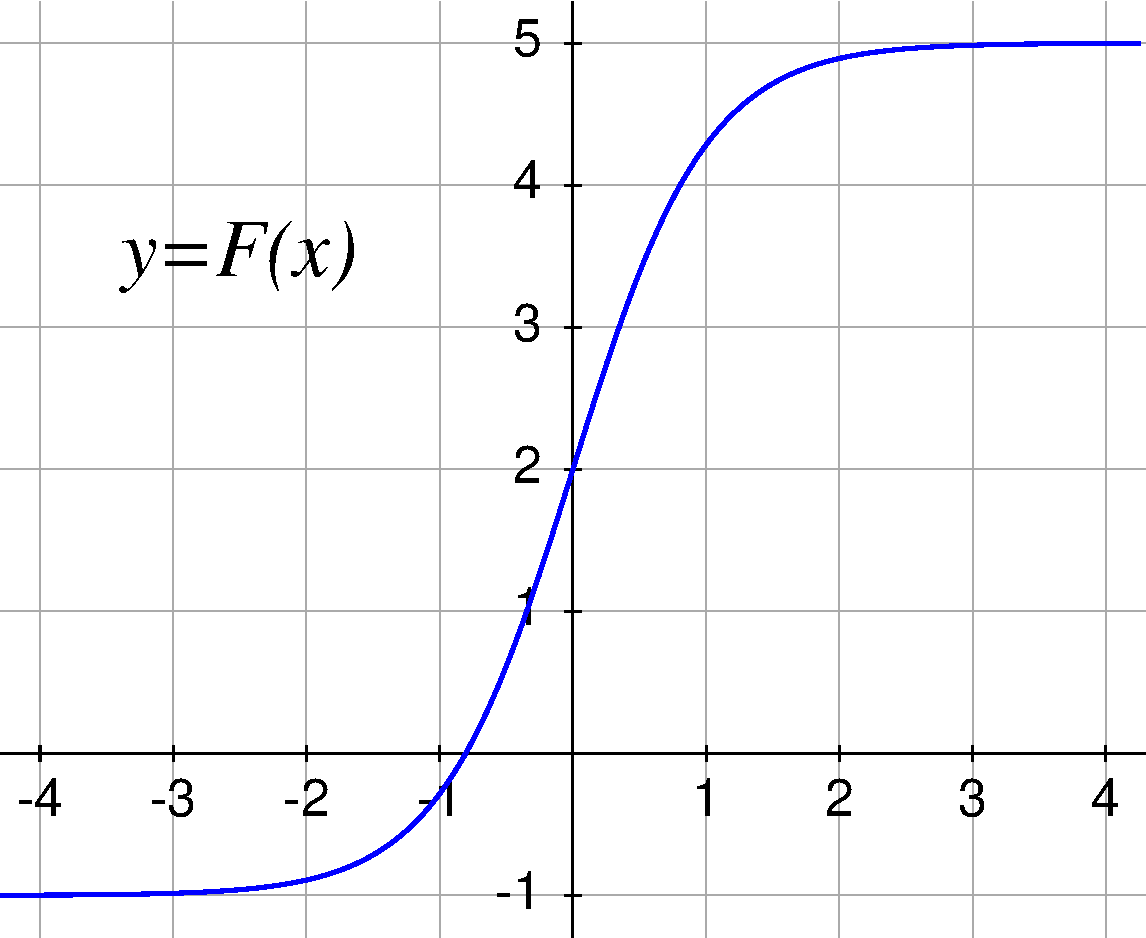
\includegraphics[scale=.29]{G15}
	\end{frame}
	%-----------------------------

	%QUESTION_INFO: {"unit":6,"question":13,"title":"Polynomial vs Exponential","images":[]}
	\begin{frame}[t]
		\frametitle{Polynomial vs Exponential}

		\begin{enumerate}
			\item Use L'H\^{o}pital Rule to compute
				\[
					\lim_{x \to \infty}\frac{x^{7}+ 5x^{3}+2}{e^{x}}
				\]

				\
			% \pause

			\item Make a conjecture for the value of
				\[
					\lim_{x \to \infty}\frac{x^{N}}{e^{x}}
				\]
				where $N$ is a positive integer. Prove it by induction.
		\end{enumerate}
	\end{frame}
	%-----------------------------

	%QUESTION_INFO: {"unit":6,"question":14,"title":"Computations","images":[]}
	\begin{frame}[t]
		\frametitle{Computations}

		Calculate:

		\begin{multicols}{2}
			\begin{enumerate}
				\item $\displaystyle \lim_{x \to 2}\frac{x^{2}+2x - 6}{x^{2}+3x-10}$

				\item $\displaystyle \lim_{x \to 0}\frac{e^{2x^2}- \cos x}{x \sin x}$

				\item $\displaystyle \lim_{x \to \infty}x^{3}e^{-x}$

				\item $\displaystyle \lim_{x \to \infty}\frac{e^{x}+ e^{-x}}{e^{x}- e^{-x}}$

				\item $\displaystyle \lim_{x \to 0}\, x \sin \frac{2}{x}$

				\item $\displaystyle \lim_{x \to \infty}x \sin \frac{2}{x}$

				\item $\displaystyle \lim_{x \to \infty}x \cos \frac{2}{x}$

				\item $\displaystyle \lim_{x \to 1}\left[ \left( \ln x \right) \tan \frac{\pi
					x}{2}\right]$
			\end{enumerate}
		\end{multicols}
	\end{frame}
	%-----------------------------

	%QUESTION_INFO: {"unit":6,"question":15,"title":"Infinity minus infinity","images":[]}
	\begin{frame}[t]
		\frametitle{Infinity minus infinity}

		Calculate:

		\begin{enumerate}
			\item $\displaystyle \lim_{x \to 0}\left[ \frac{\csc x}{x}- \frac{\cot x}{x}
				\right]$

				\

			\item $\displaystyle \lim_{x \to \infty}\left[ \ln (x+2) - \ln(3x+4) \right
				]$

				\

			\item $\displaystyle \lim_{x \to 1}\left[ \frac{2}{x^{2}-1}- \frac{1}{x-1}\right
				]$

			\item $\displaystyle \lim_{x \to - \infty}\left[ \sqrt{x^{2}+3x}- \sqrt{x^{2}-3x}
				\right]$
		\end{enumerate}
	\end{frame}
	%-----------------------------

	%QUESTION_INFO: {"unit":6,"question":16,"title":"Exponential indeterminate forms","images":[]}
	\begin{frame}[t]
		\frametitle{Exponential indeterminate forms}

		Calculate:

		\begin{enumerate}
			\item $\displaystyle \lim_{x \to 0}\left[ 1 + 2 \sin(3x) \right]^{4 \cot (5x)}$

			\item $\displaystyle \lim_{x \to \infty }\left( \frac{x+2}{x-2}\right)^{3x}$

			\item $\displaystyle \lim_{x \to 0^+}x^{x}$

			\item $\displaystyle \lim_{x \to {\frac{\pi}{2}}^{-}}\left( \tan x \right)^{\cos
				x}$

			\item $\displaystyle \lim_{x \to 0}\left( \frac{\sin x}{x}\right)^{1 /x^2}$
		\end{enumerate}
	\end{frame}
	%-----------------------------

	%QUESTION_INFO: {"unit":6,"question":17,"title":"Backwards L’Hôpital","images":[]}
	\begin{frame}[t]
		\frametitle{Backwards L'H\^{o}pital}

		Construct a polynomial $P$ such that
		\[
			\lim_{x \to 1}\; \frac{P(x)}{e^{x}- e \cdot x}\; = \; \frac{1}{e}
		\]
	\end{frame}

	%-----------------------------

	%QUESTION_INFO: {"unit":6,"question":18,"title":"Come to the dark side","images":[]}
	\begin{frame}[t]
		\fontsize{13}{13}\selectfont
		\frametitle{Come to the dark side}

		Help us write a difficult question for Test 3! We will ask you to compute a
		limit like this
		\[
			\lim_{x \to 0}\frac{e^{x}+ e^{-x}- 2 \cos x + bx^{N}}{x^{6}}
		\]
		where $b$ is a real number and $N$ is a natural number that we have not
		chosen yet.

		We do not want the answer to be $0$ or $\infty$ or $-\infty$ or ``DNE",
		because you could guess that randomly.

		What values of $b$ and $N$ should we choose? What will the value of the limit
		be?
	\end{frame}
	%-----------------------------

	%QUESTION_INFO: {"unit":6,"question":19,"title":"Indeterminate?","images":[]}
	\begin{frame}[t]
		\frametitle{Indeterminate?}

		Which of the following are indeterminate forms for limits? \\ If any of them
		isn't, then what is the value of such limit?

		\begin{multicols}{4}
			\begin{enumerate}
				\setlength{\itemsep}{1em}

				\item $\displaystyle \frac{0}{0}$

				\item $\displaystyle \frac{0}{\infty}$

				\item $\displaystyle \frac{0}{1}$

				\item $\displaystyle \frac{\infty}{0}$

				\item $\displaystyle \frac{\infty}{\infty}$

				\item $\displaystyle \frac{1}{\infty}$

				\item $\displaystyle 0 \cdot \infty$ \phantom{$\displaystyle \frac{1}{1}$}

				\item $\displaystyle \infty \cdot \infty$ \phantom{$\displaystyle \frac{1}{1}$}

				\item $\displaystyle \sqrt{\infty}$

				\item $\displaystyle \infty - \infty$

				\item $\displaystyle 1^{\infty}$

				\item $\displaystyle 1^{-\infty}$

				\item $\displaystyle 0^{0}$

				\item $\displaystyle 0^{\infty}$

				\item $\displaystyle 0^{-\infty}$

				\item $\displaystyle \infty^{0}$

				\item $\displaystyle \infty^{\infty}$

				\item $\displaystyle \infty^{-\infty}$
			\end{enumerate}
		\end{multicols}
	\end{frame}
	%-----------------------------

	%QUESTION_INFO: {"unit":6,"question":20,"title":"Proving something is an indeterminate form","images":[]}
	\begin{frame}[t]
		\fontsize{13}{13}\selectfont
		\frametitle{Proving something is an indeterminate form}

		\begin{enumerate}
			\item Prove that $\displaystyle \forall c \in \mathbb{R}$,
				$\displaystyle \exists a \in \mathbb{R}$ and functions $f$ and $g$ such
				that
				\[
					\lim_{x \to a}f(x) = 0, \quad \lim_{x \to a}g(x) =0, \quad \lim_{x \to
					a}\frac{f(x)}{g(x)}= c
				\]

				This is how you show that $\displaystyle \frac{0}{0}$ is an indeterminate
				form.

				\
			% \pause

			\item Prove the same way that $\displaystyle \frac{\infty}{\infty}$,
				$\displaystyle 0 \cdot \infty$, and $\displaystyle \infty - \infty$ are also
				indeterminate forms.

				\
			% \pause

			\item Prove that $\displaystyle 1^{\infty}$, $\displaystyle 0^{0}$, and $\displaystyle
				\infty^{0}$ are indeterminate forms.

				(You will only get $c \geq 0$ this time)
		\end{enumerate}
	\end{frame}
	%-----------------------------

	%----------------------------------------------------------------------------------------

	%	Concavity, asymptotes, and graphing

	%----------------------------------------------------------------------------------------

	%-----------------------------

	%QUESTION_INFO: {"unit":6,"question":21,"title":"Find the coordinates of $P$ and $Q$","images":["G16.svg","G16.pdf"]}
	\begin{frame}[t]
		\frametitle{Find the coordinates of $P$ and $Q$}
		\vspace{-.5cm}
		\[
			g(x) = x^{4}- 6x^{2}+ 9
		\]

		\begin{center}
			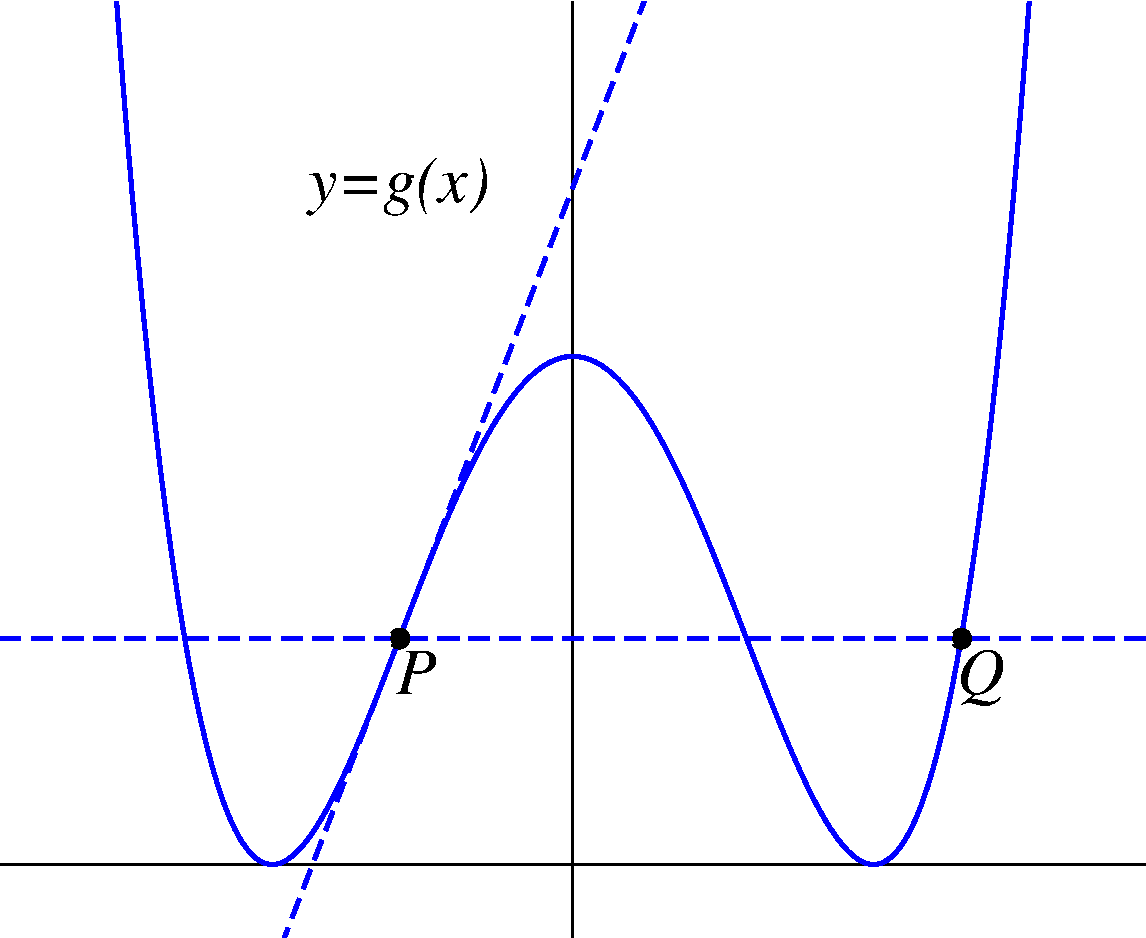
\includegraphics[scale=.4]{G16}
		\end{center}
	\end{frame}
	%-----------------------------

	%QUESTION_INFO: {"unit":6,"question":22,"title":"Find the coordinates of $P$ ","images":["G17.pdf"]}
	\begin{frame}[t]
		\frametitle{Find the coordinates of $P$ }

		\[
			f(x) = 3x+4 + \frac{2x-10}{x^{2}}
		\]

		\begin{center}
			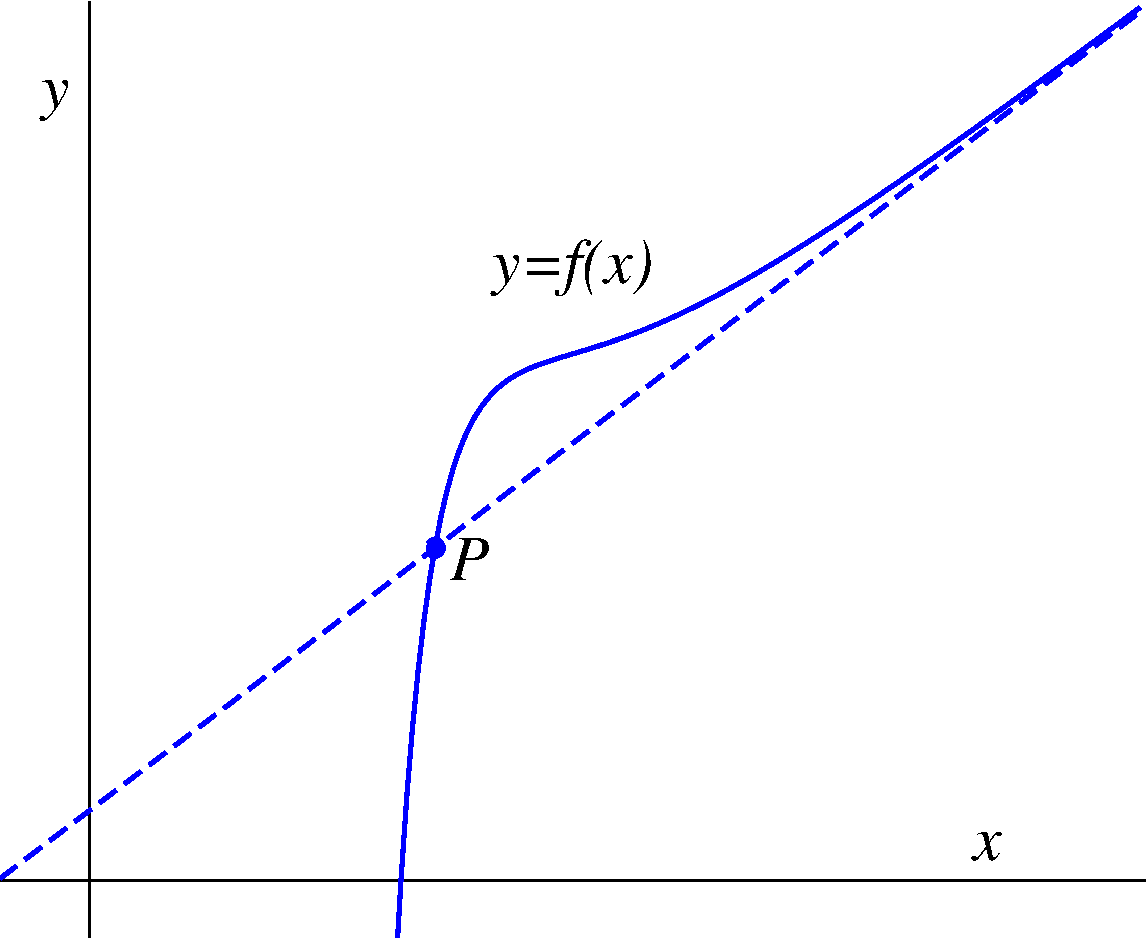
\includegraphics[scale=0.4]{G17}
		\end{center}
	\end{frame}
	%-----------------------------

	%QUESTION_INFO: {"unit":6,"question":23,"title":"True or False — Concavity and inflection points","images":[]}
	\begin{frame}[t]
		\fontsize{13}{13}\selectfont
		\frametitle{True or False -- Concavity and inflection points}

		Let $f$ be a {{differentiable}} function with domain $\mathbb{R}$. \\ Let
		$c \in \mathbb{R}$. Let $I$ be an interval. Which implications are true?

		\begin{enumerate}
			\item IF {\color{red} $f$ is concave up on $I$}, \quad THEN
				{\color{blue} $\forall x \in I$, $f''(x) >0$}.

			\item IF {\color{blue} $\forall x \in I$, $f''(x) >0$}, \quad THEN
				{\color{red} $f$ is concave up on $I$}.

			\item IF {\color{red} $f$ is concave up on $I$} \quad THEN {\color{verde} $f'$ is increasing on $I$}.

			\item IF {\color{verde} $f'$ is increasing on $I$}, \quad THEN
				{\color{red} $f$ is concave up on $I$}.

			\item IF {\color{rosa} $f$ has an I.P.\ at $c$}, \quad THEN
				{\color{naranja} $f''(c)=0$}.

			\item IF {\color{naranja} $f''(c)=0$}, \quad THEN
				{\color{rosa} $f$ has an I.P.\ at $c$}.

			\item IF {\color{rosa} $f$ has an I.P. at $c$}, \quad THEN
				{\color{violet} $f'$ has a local extremum at $c$}

			\item IF {\color{violet} $f'$ has a local extremum at $c$}, \quad THEN
				{\color{rosa} $f$ has an I.P.\ at $c$}.
		\end{enumerate}
		\begin{center}
			I.P.\  = ``inflection point"
		\end{center}
	\end{frame}
	%-----------------------------

	%QUESTION_INFO: {"unit":6,"question":24,"title":"“Secant segments are above the graph”","images":[]}
	\begin{frame}[t]
		\fontsize{13}{13}\selectfont
		\frametitle{``Secant segments are above the graph"}

		Let $f$ be a function defined on an interval $I$.\\ In Video 6.13 you learned
		that an alternative to our definition of ``$f$ is concave up on $I$" is ``the
		secant segments stay above the graph".

		\begin{center}
			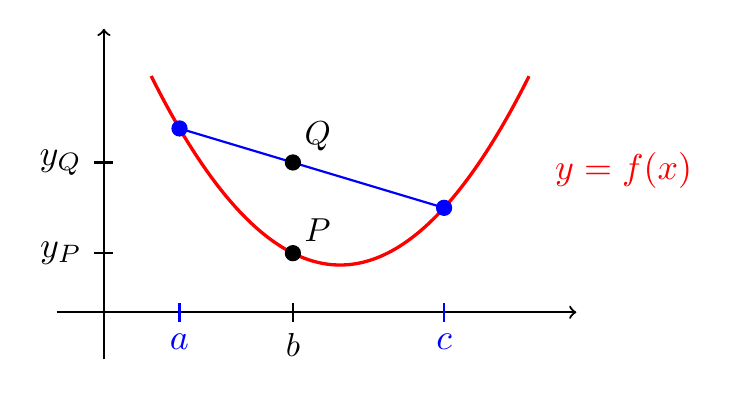
\begin{tikzpicture}[scale=1.2]
				\draw[thick, ->] (-0.5,0) -- (5,0);
				\draw[thick, ->] (0,-0.5) -- (0,3);
				\draw[
					domain=0.5:4.5,
					smooth,
					variable=\x,
					samples={200},
					red,
					very thick
				] plot ({\x}, {(\x-2.5)*(\x-2.5)/2 + .5});
				\node[red, scale=1.3] at (5.5,1.5) {$\displaystyle y=f(x)$};
				\draw[blue, fill] (.8,1.945) circle[radius=0.08];
				\draw[blue, fill] (3.6,1.105) circle[radius=0.08];
				\draw[thick, blue] (.8,-.1) to (.8,.1);
				\node[below, blue, scale=1.3] at (.8,-.1) {$a$};
				\draw[thick, blue] (3.6,-.1) to (3.6,.1);
				\node[below, blue, scale=1.3] at (3.6,-.1) {$c$};
				\draw[blue, thick] (.8,1.945) -- (3.6,1.105);
				\draw[thick] (2,-.1) to (2,.1);
				\node[below, black, scale=1.2] at (2,-.1) {$b$};
				\draw[black, fill] (2,0.625) circle[radius=0.08];
				\node[above right, black, scale=1.2] at (2,0.625) {$P$};
				\draw[black, fill] (2,1.585) circle[radius=0.08];
				\node[above right, black, scale=1.2] at (2,1.585) {$Q$};
				\draw[thick] (-.1,0.625) to (.1,.625);
				\node[left, black, scale=1.3] at (-.1,0.625) {$y_{P}$};
				\draw[thick] (-.1,1.585) to (.1,1.585);
				\node[left, black, scale=1.3] at (-.1,1.585) {$y_{Q}$};
			\end{tikzpicture}
		\end{center}

		Rewrite this as a precise mathematical statement of the form
		\[
			``\forall a,b,c \in I, \quad a<b<c \; \implies \; \boxed{\text{an inequality involving $f$, $a$, $b$, $c$}}
			"
		\]
	\end{frame}
	%-----------------------------

	%QUESTION_INFO: {"unit":6,"question":25,"title":"A polynomial from 3 points","images":[]}
	\begin{frame}[t]
		\frametitle{A polynomial from 3 points}

		Construct a polynomial that satisfies the following three properties at once:
		\begin{enumerate}
			\item It has an inflection point at $x=2$

			\item It has a a local extremum at $x=1$

			\item It has $y$-intercept at $y=1$.
		\end{enumerate}
	\end{frame}

	%-----------------------------

	%QUESTION_INFO: {"unit":6,"question":26,"title":"Monotonicity and concavity","images":[]}
	\begin{frame}[t]
		\frametitle{Monotonicity and concavity}

		Let $\displaystyle f(x) = x e^{-x^2/2}$.

		\begin{enumerate}
			\item Find the intervals where $f$ is increasing or decreasing, and its
				local extrema.

			\item Find the intervals where $f$ is concave up or concave down, and its
				inflection points.

			\item Calculate $\displaystyle \lim_{x \to \infty}f(x)$ and $\displaystyle
				\lim_{x \to - \infty}f(x)$.

			\item Using this information, sketch the graph of $f$.
		\end{enumerate}
	\end{frame}
	%-----------------------------

	%QUESTION_INFO: {"unit":6,"question":27,"title":"Fractional exponents","images":[]}
	\begin{frame}[t]
		\frametitle{Fractional exponents}

		Let $\displaystyle h(x) = \frac{x^{2/3}}{(x-1)^{2/3}}$. Its first two derviatives
		are
		\begin{equation*}
			h'(x) = \frac{-2}{3x^{1/3}(x-1)^{5/3}}\; \quad \quad h''(x) = \frac{2(6x-1)}{9x^{4/3}(x-1)^{8/3}}
		\end{equation*}

		\begin{enumerate}
			\item Find all asymptotes of $h$

			\item Study the monotonicity of $h$ and local extrema

			\item Study the concavity of $h$ and inflection points

			\item With this information, sketch the graph of $h$
		\end{enumerate}
	\end{frame}
	%-----------------------------

	%QUESTION_INFO: {"unit":6,"question":28,"title":"Hyperbolic tangent","images":[]}
	\begin{frame}[t]
		\frametitle{Hyperbolic tangent}

		The function $\tanh$, defined by
		\[
			\tanh x = \frac{e^{x}- e^{-x}}{e^{x}+ e^{-x}},
		\]
		is called the ``hyperbolic tangent".
		\begin{enumerate}
			\item Find its two asymptotes

			\item Study its monotonicity

			\item Study its concavity

			\item With this information, sketch its graph.
		\end{enumerate}
	\end{frame}
	%-----------------------------

	%QUESTION_INFO: {"unit":6,"question":29,"title":"A very hard function to graph","images":[]}
	\begin{frame}[t]
		\frametitle{A very hard function to graph}

		The function $\displaystyle G(x) = x e^{1/x}$ is deceiving. To help you out:
		\[
			G'(x) = \frac{x-1}{x}e^{1/x}, \quad \quad G''(x) = \frac{e^{1/x}}{x^{3}}
		\]

		\begin{enumerate}
			\item Carefully study the behaviour as $x \to \pm \infty$. \\ You should
				find an asymptote, but it is not easy.

			\item Carefully study the behaviour as $x \to 0^{+}$ and $x\to 0^{-}$. The
				two are very different.

			\item Use $G'$ to study monotonocity.

			\item Use $G''$ to study concavity.

			\item Sketch the graph of $G$.
		\end{enumerate}
	\end{frame}

	%-----------------------------

	%QUESTION_INFO: {"unit":6,"question":30,"title":"Backwards graphing ","images":["G19.svg","G19.png"]}
	\begin{frame}[t]
		\frametitle{Backwards graphing }

		$R$ is a rational function (a quotient of polynomials). \\ Find its equation.
		\begin{center}
			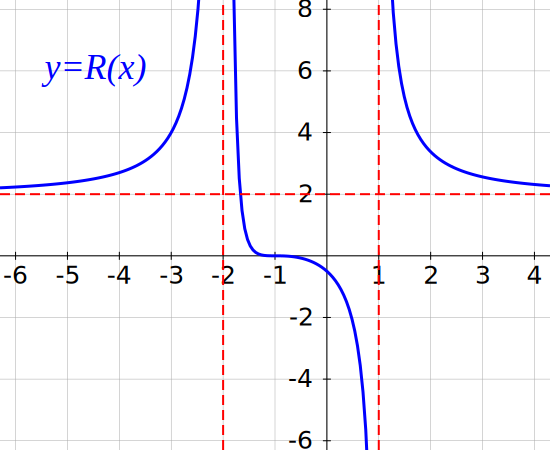
\includegraphics[scale=.4]{G19}
		\end{center}
	\end{frame}

	%-----------------------------

	%QUESTION_INFO: {"unit":6,"question":31,"title":"Unexpected asymptotes","images":[]}
	\begin{frame}[t]
		\frametitle{Unexpected asymptotes}

		Find the two asymptotes of the function
		\[
			F(x) = x + \sqrt{x^{2}+2x+ 2}
		\]

		\emph{Hint:} The behaviour as $x \to \infty$ is very different from
		$x \to - \infty$.

		\ \hfill \href{https://www.desmos.com/calculator/kffnbl6pnc}{\beamergotobutton{graph}}
	\end{frame}

	%-----------------------------

	%QUESTION_INFO: {"unit":6,"question":32,"title":"Unusual examples","images":[]}
	\begin{frame}[t]
		\frametitle{Unusual examples}

		Construct three functions $f$, $g$, and $h$.

		\begin{enumerate}
			\item $f$ has domain at least $(0,\infty)$, is continuous, is always concave
				up, and satisfies $\displaystyle \lim_{x \to \infty}f(x) = - \infty$

			\item $g$ has domain $\mathbb{R}$, is continuous, has a local minimum at $x
				=0$, and has an inflection point also at $x=0$.

			\item $h$ has domain $\mathbb{R}$, is differentiable, is strictly increasing.
				In addition, $h'$ is periodic with period $2$, and $h'$ is not constant.
		\end{enumerate}
	\end{frame}
	%-----------------------------

	%-----------------------------

	%-----------------------------
\end{document}
%-----------------------------

%-----------------------------